\documentclass[conference]{IEEEtran}

\usepackage{booktabs}
\usepackage{tabularx}
\usepackage{array}
\usepackage{amsmath}
\usepackage{url}
\usepackage{xcolor}
\usepackage{enumitem}
\usepackage{graphicx}
\usepackage[hidelinks]{hyperref}

\graphicspath{{figures/}}

\title{Can Sovereign Wealth Fund Disclosures Be Monetized?\\
A Disclosure-Lag-Aware Study of PIF and Norges Bank Signals}

\author{
\IEEEauthorblockN{Ethan Wei}
\IEEEauthorblockA{Independent Research Project\\
Singapore\\
\texttt{ethanwei6}}
}

\begin{document}
\maketitle

\begin{abstract}
This paper examines whether public sovereign wealth fund (SWF) disclosures contain investable information once disclosure lag, partial visibility, and implementation constraints are treated as first-class design variables. The project began with three funds---Saudi Arabia's Public Investment Fund (PIF), Norges Bank Investment Management (NBIM), and Singapore's GIC---but quickly encountered radical disclosure asymmetry: NBIM provides broad but slow public-equity visibility, PIF provides security-level visibility only for its reportable U.S. 13F sleeve, and GIC is too opaque to support a comparable holdings panel. We therefore construct fund-specific normalized datasets and test lag-aware strategies rather than forcing all funds into a common template.

For PIF, five backtests are implemented on a canonical 13F panel with filing-aware trade timing, benchmark comparison against \texttt{SPY}, and a corrected split-adjusted price layer. After validation, all strategies underperform on an excess-return basis; the best cash-aware variant still trails the benchmark materially. For NBIM, eight strategies are tested against \texttt{VT} using split-adjusted daily prices for first-post-release execution and month-end marks derived from the same daily source. The strongest direct mirror results are shown to be contaminated by survivor-selection in a bounded mega-cap universe. More credible sector-based tests produce only modest benchmark-relative gains, with the best results coming from industry weight-change and concentrated leadership strategies. Across both funds, the evidence does not support strong claims of easy copy-trading alpha. The most credible signal is slower-moving sector posture rather than single-name imitation.
\end{abstract}

\begin{IEEEkeywords}
sovereign wealth funds, 13F, NBIM, PIF, disclosure lag, backtesting, sector rotation, alpha
\end{IEEEkeywords}

\section{Introduction}

Large sovereign wealth funds (SWFs) are unusual public investors. They are patient, structurally large, politically salient, and often treated by market participants as ``strong hands'' rather than tactical traders. This creates an intuitive hypothesis: if SWFs are informed, patient allocators, perhaps public disclosure of their holdings or reallocations contains tradable information.

That simple hypothesis becomes difficult once one confronts the actual disclosure regimes. Some funds disclose broad holdings but at long lag; others disclose only narrow regulatory subsets; others remain too opaque to support a serious panel. This project was designed around that asymmetry rather than around an idealized ``all funds disclose the same thing'' assumption.

The original target funds were:
\begin{itemize}[leftmargin=1.4em]
    \item \textbf{NBIM}, manager of Norway's Government Pension Fund Global;
    \item \textbf{PIF}, Saudi Arabia's Public Investment Fund; and
    \item \textbf{GIC}, Singapore's sovereign wealth fund.
\end{itemize}

The original research questions were:
\begin{enumerate}[leftmargin=1.4em]
    \item Can an investor harvest alpha by mirroring disclosed SWF positions after the information becomes public?
    \item If single-name mirroring fails, can alpha still be extracted from the sectors or industries into which SWFs are rotating?
    \item Are observable exits or reductions structured enough to improve timing or reduce stale-trade risk?
\end{enumerate}

The project ultimately contributes four things:
\begin{enumerate}[leftmargin=1.4em]
    \item a disclosure-aware research design for heterogeneous SWF datasets;
    \item normalized holdings, transition, and benchmark layers for PIF and NBIM;
    \item validated lag-aware backtests distinguishing exploratory from credible results; and
    \item reproducible reports, charts, and interactive artifacts that expose the full path from disclosure to simulated trade.
\end{enumerate}

\section{Research Scope and Disclosure Regimes}

\subsection{Core Principle}

The governing design rule was:
\begin{quote}
\textit{A signal may only be traded after it is public, and no backtest may use a portfolio effective date as a trade date unless it is also the public date.}
\end{quote}

This rule is the main protection against overstated alpha in disclosure-based research.

\subsection{Disclosure Regimes}

Table~\ref{tab:disclosure} summarizes the three target funds.

\begin{table}[!t]
\caption{Disclosure Regimes Across Target Funds}
\label{tab:disclosure}
\centering
\begin{tabularx}{\columnwidth}{>{\raggedright\arraybackslash}p{1.4cm} >{\raggedright\arraybackslash}p{2.2cm} X}
\toprule
\textbf{Fund} & \textbf{Primary Public Source} & \textbf{Research Implication} \\
\midrule
NBIM & Public holdings database plus annual / half-year reports & Broad public-equity coverage, but low timeliness; suitable for slow-moving portfolio and industry tests. \\
PIF & SEC 13F filings & Security-level visibility with filing dates, share counts, and values; strongest candidate for lagged mirroring tests. \\
GIC & Annual reports and sparse external ownership filings & Too opaque for a comparable holdings panel; retained as a qualitative disclosure-asymmetry case. \\
\bottomrule
\end{tabularx}
\end{table}

The final quantitative panel therefore excludes GIC, not because the fund is unimportant, but because the public data was too thin to support a comparable holdings backtest without false precision \cite{gicreports,gicsantiago}.

\section{Data Construction Pipeline}

\subsection{Data Layers}

The project was built around reusable data layers rather than one-off spreadsheets:
\begin{itemize}[leftmargin=1.4em]
    \item \textbf{Holdings panels:} normalized security or issuer snapshots.
    \item \textbf{Transition panels:} entries, exits, and change classifications between snapshots.
    \item \textbf{Summary panels:} sector, geography, and concentration summaries by period.
    \item \textbf{Backtest outputs:} signal eligibility, rebalance events, order blotters, position histories, portfolio paths, and benchmark-relative summaries.
\end{itemize}

\subsection{Dataset Scale}

The final project scale is summarized in Table~\ref{tab:dataset-scale}.

\begin{table}[!t]
\caption{Dataset Scale After Cleaning}
\label{tab:dataset-scale}
\centering
\begin{tabularx}{\columnwidth}{>{\raggedright\arraybackslash}p{1.0cm} >{\raggedright\arraybackslash}p{1.7cm} >{\raggedright\arraybackslash}p{1.5cm} X}
\toprule
\textbf{Fund} & \textbf{Holdings Rows} & \textbf{Periods} & \textbf{Additional Scale Information} \\
\midrule
PIF & 775 & 30 & 30 canonical filings, 6 amendments in raw set, 998 transition rows, 88 priced securities. \\
NBIM & 97{,}010 & 11 & 98{,}450 transition rows, 16{,}445 unique issuer-country keys, 20 priced instruments plus 2 explicitly missing ETF proxies. \\
\bottomrule
\end{tabularx}
\end{table}

\subsection{PIF Data Pipeline}

PIF data was pulled from EDGAR 13F filing folders containing \texttt{primary\_doc.xml} and \texttt{informationtable.xml}, consistent with the SEC's 13F disclosure framework \cite{sec13f}. The pipeline:
\begin{enumerate}[leftmargin=1.4em]
    \item parsed filing metadata and holdings rows from XML,
    \item indexed amendments and canonical filing versions,
    \item normalized security keys using CUSIP, class, and option flags,
    \item built a transition dataset based on share-count and value changes, and
    \item mapped approved securities to a validated price layer.
\end{enumerate}

The transition dataset classified \texttt{entry\_observed}, \texttt{exit\_observed}, \texttt{likely\_accumulation}, \texttt{likely\_reduction}, and \texttt{continued\_holding}. Because 13F includes share counts, these classifications could be anchored in actual share changes rather than inferred ownership percentages.

\subsection{NBIM Data Pipeline}

NBIM data was assembled from downloaded public equity files labeled by snapshot date (e.g., \texttt{eq\_YYYYMMDD}) using NBIM's public holdings distribution \cite{nbim,nbimholdings}. The pipeline:
\begin{enumerate}[leftmargin=1.4em]
    \item stacked semicolon-delimited holdings files into a consolidated issuer-level panel,
    \item normalized numeric ownership and voting fields,
    \item generated annual and half-year summary datasets,
    \item classified issuer transitions between snapshots, and
    \item mapped industry exposures to liquid U.S. sector ETF proxies.
\end{enumerate}

Unlike PIF, NBIM holdings did not include share counts. This matters. A change in market value alone does not prove buying or selling. Therefore, the NBIM transition engine treated inclusion/exclusion and ownership-percentage changes as the strongest available indicators and did not infer flows directly from value movement.

\subsection{GIC Treatment}

GIC remained in scope conceptually but out of scope for the quantitative backtests. The project documented the relevant proxy channels---major-shareholder filings, 13D/G, HKEX DI, FCA TR-1, EDINET, and deal press---but did not construct a comparable holdings panel because the public evidence was episodic, threshold-driven, and structurally incomplete.

\section{Price Layers, Benchmarks, and Trade Timing}

\subsection{Trade Timing}

All strategies obeyed disclosure-lag-aware execution rules:
\begin{itemize}[leftmargin=1.4em]
    \item \textbf{PIF signal date:} SEC public filing date.
    \item \textbf{PIF trade date:} next trading day after the public date.
    \item \textbf{NBIM signal date:} official annual or half-year publication date.
    \item \textbf{NBIM trade date:} first tradable close strictly after publication.
\end{itemize}

For NBIM, the portfolio is rebalanced at the first post-release daily close and then carried at month-end closes until the next report. This preserves realistic post-disclosure reaction timing without requiring full daily path simulation between reports.

\subsection{Benchmarks}

The benchmark selection matched the disclosed universe:
\begin{itemize}[leftmargin=1.4em]
    \item \textbf{PIF benchmark:} \texttt{SPY}, reflecting a U.S.-listed 13F sleeve.
    \item \textbf{NBIM benchmark:} \texttt{VT}, reflecting a broad global public-equity owner.
\end{itemize}

\subsection{Price Sources}

Price infrastructure was fund-specific:
\begin{itemize}[leftmargin=1.4em]
    \item \textbf{PIF:} Twelve Data daily price history, with both raw execution prices and an adjusted mark-to-market layer \cite{twelvedata}.
    \item \textbf{NBIM:} Twelve Data adjusted daily history for the benchmark, ETF proxies, and the bounded direct mirror universe; month-end marks are derived from this daily source \cite{twelvedata}.
\end{itemize}

This unified daily source removed the earlier timing distortion from waiting until the next month-end to enter an NBIM trade and also eliminated the earlier ETF proxy gaps.

\section{Strategy Definitions}

\subsection{PIF Strategies}

Five PIF strategies were tested:
\begin{enumerate}[leftmargin=1.4em]
    \item \textbf{P1 New Positions Mirror:} buy new disclosed entries only.
    \item \textbf{P2 Full Sleeve Equal Weight:} hold the full common-equity 13F sleeve equally weighted.
    \item \textbf{P3 Accumulation Tilt:} overweight likely accumulations.
    \item \textbf{P4 Exit Avoidance:} avoid likely reductions and exits.
    \item \textbf{P5 Cash-Aware Copy:} copy buys and sells as disclosed while retaining sale proceeds in cash.
\end{enumerate}

P5 was introduced after an important conceptual observation: if PIF liquidates positions from its disclosed sleeve, a literal copycat should often keep the residual cash rather than mechanically concentrating the survivors.

\subsection{NBIM Strategies}

NBIM strategies naturally fall into two families.

\subsubsection{Exploratory direct mirrors}
\begin{enumerate}[leftmargin=1.4em]
    \item \textbf{N1 Core U.S. Mirror Equal Weight}
    \item \textbf{N2 Core U.S. Mirror NBIM Weight}
\end{enumerate}

These were included because single-name mirroring was one of the original hypotheses, but they rely on a bounded U.S. mirror sleeve rather than a full global book.

\subsubsection{Industry-based strategies}
\begin{enumerate}[leftmargin=1.4em]
    \item \textbf{N3 Industry Weight Mirror:} reproduce the disclosed industry posture through ETF proxies.
    \item \textbf{N4 Industry Weight-Change Tilt:} hold only sectors whose disclosed weights increased versus the prior snapshot.
    \item \textbf{N5 Industry Accumulation Tilt:} hold sectors with positive accumulation-minus-reduction transition scores.
    \item \textbf{N6 Top-3 Industry Leaders:} concentrate in the three largest disclosed sector exposures.
    \item \textbf{N7 Top-3 Industry Increases:} hold the three largest positive sector changes.
    \item \textbf{N8 Consensus Rotation Tilt:} require both positive weight change and positive transition score.
\end{enumerate}

This second family is more realistic and more aligned with what NBIM actually discloses: slow-moving sector posture rather than actionable stock-level trading instructions.

\subsection{Benchmark-Relative Measure}

For clarity, the paper reports both standalone total return and benchmark-relative excess return. The latter is defined as
\begin{equation}
R^{\text{excess}}_{s,T}=\frac{\text{NAV}_{s,T}/\text{NAV}_{s,0}}{\text{NAV}_{b,T}/\text{NAV}_{b,0}}-1,
\end{equation}
where $s$ is the strategy and $b$ is the benchmark. This choice makes the interpretation straightforward: positive values represent outperformance over the matched benchmark horizon.

\section{Validation Protocol}

\subsection{Why Validation Changed the Interpretation}

The project produced two major validation lessons.

\subsubsection{PIF split handling}

Early PIF results appeared dramatically positive. Investigation showed that raw close series were being marked against unchanged share counts through reverse splits, creating fake gains. Once the backtests were rebuilt on adjusted mark-to-market pricing, the apparent alpha disappeared and all fully invested PIF strategies became negative in benchmark-relative terms.

\subsubsection{NBIM mirror-universe bias}

The initial NBIM direct mirror results were also strikingly positive, but the issue was different. Here the arithmetic was fine; the interpretation was not. The bounded mirror universe turned out to be almost the same recurring basket of U.S. mega-cap winners in every snapshot. A mirror strategy built on that sleeve is closer to a hand-selected winners basket than to a neutral test of disclosure alpha.

\subsection{Mechanical Integrity Checks}

The final backtests were checked for:
\begin{itemize}[leftmargin=1.4em]
    \item negative cash breaches,
    \item impossible gross exposure,
    \item weight-integrity gaps, and
    \item rebalance arithmetic consistency.
\end{itemize}

For the final NBIM panel, all strategies showed zero negative-cash breaches and only floating-point-level weight gaps. The corrected PIF engines passed the same integrity standard.

\section{Results: PIF}

\subsection{Summary Results}

Table~\ref{tab:pif-results} reports the validated PIF strategy outcomes. The important point is not just that most strategies fail, but that the \emph{best conceptual fix} (cash-aware copying) still fails to generate alpha versus the benchmark.

\begin{table*}[!t]
\caption{PIF Strategy Results versus SPY}
\label{tab:pif-results}
\centering
\begin{tabular}{lrrrrr}
\toprule
\textbf{Strategy} & \textbf{Total Return} & \textbf{CAGR} & \textbf{Max Drawdown} & \textbf{Excess Return vs SPY} & \textbf{Information Ratio} \\
\midrule
P1 New Positions Mirror & $-75.8\%$ & $-20.2\%$ & $-94.8\%$ & $-90.5\%$ & $-0.299$ \\
P2 Full Sleeve Equal Weight & $-32.3\%$ & $-5.2\%$ & $-81.1\%$ & $-77.4\%$ & $-0.319$ \\
P3 Accumulation Tilt & $-69.3\%$ & $-15.0\%$ & $-88.7\%$ & $-89.8\%$ & $-0.415$ \\
P4 Exit Avoidance & $-45.2\%$ & $-7.9\%$ & $-80.9\%$ & $-81.7\%$ & $-0.362$ \\
P5 Cash-Aware Copy & $+48.9\%$ & $+5.6\%$ & $-62.6\%$ & $-50.4\%$ & $-0.120$ \\
\bottomrule
\end{tabular}
\end{table*}

\begin{figure*}[!t]
\centering
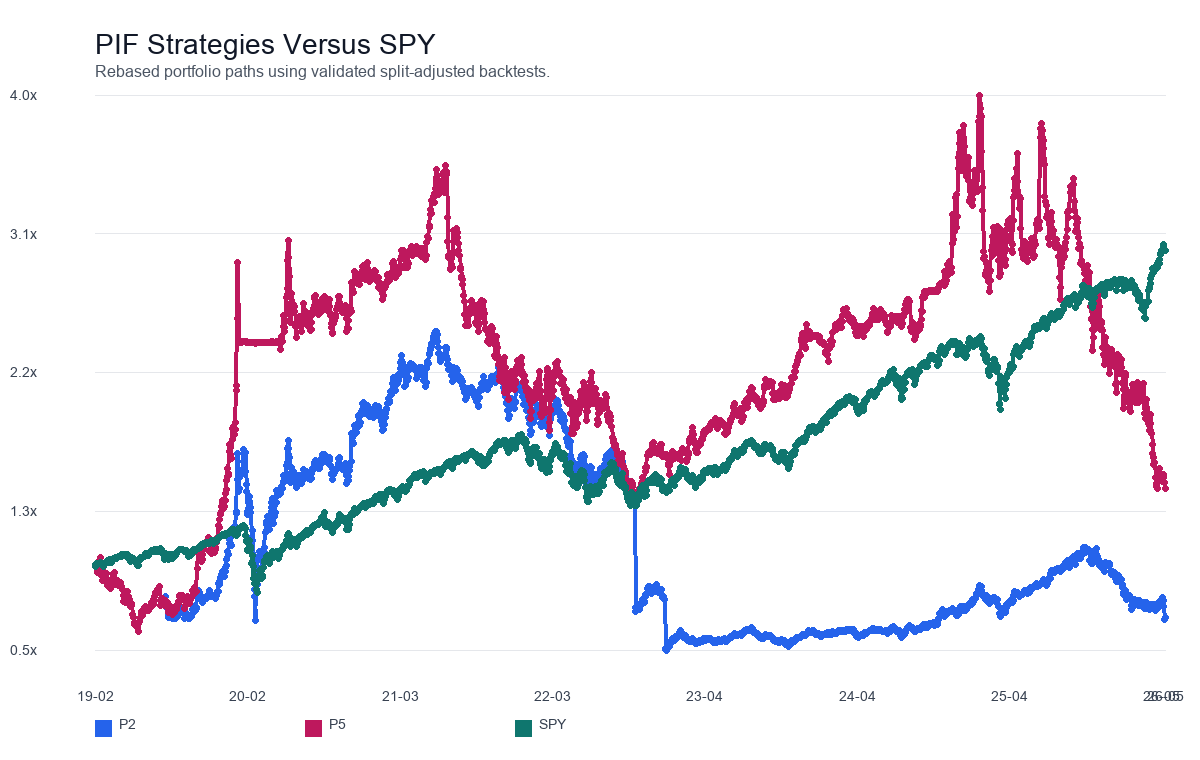
\includegraphics[width=0.92\textwidth]{pif_nav_vs_spy.png}
\caption{Validated PIF strategy paths versus SPY. The cash-aware strategy (P5) materially improves on fully invested variants but still lags the benchmark.}
\label{fig:pif-nav}
\end{figure*}

\begin{figure}[!t]
\centering
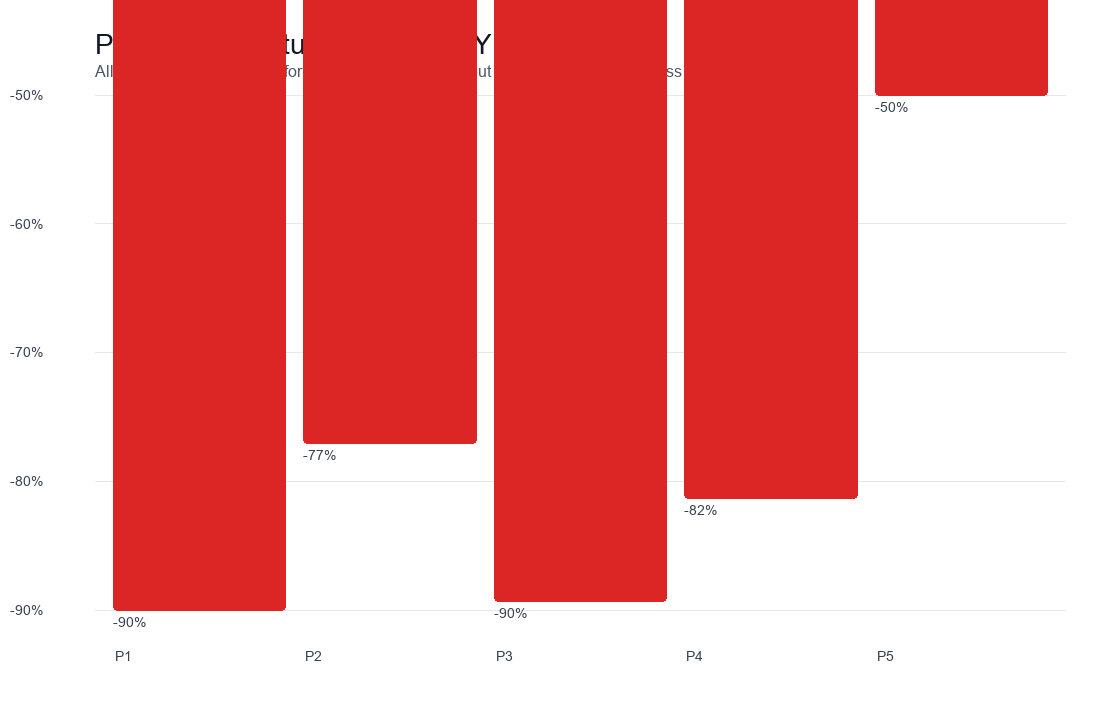
\includegraphics[width=\columnwidth]{pif_excess_return.png}
\caption{Excess total return of PIF strategies versus SPY.}
\label{fig:pif-excess}
\end{figure}

\subsection{Interpretation}

Three findings are robust:
\begin{enumerate}[leftmargin=1.4em]
    \item \textbf{Naive mirroring fails.} Security-level lagged copying of the disclosed 13F sleeve is not a strong stock-picking edge.
    \item \textbf{Cash-awareness helps but does not rescue alpha.} The difference between P2--P4 and P5 shows that disclosed sales contain useful exposure information, but not enough to beat passive U.S. beta.
    \item \textbf{Partial disclosure is a structural limit.} Even a mechanically faithful mirror of PIF's 13F book is not a mirror of the entire fund.
\end{enumerate}

The implication is that PIF's public sleeve is better interpreted as a monitoring and posture dataset than as a direct alpha source.

\section{Results: NBIM}

\subsection{Exploratory Mirrors versus Realistic Signals}

Table~\ref{tab:nbim-results} reports the final NBIM strategy results versus \texttt{VT}. Unlike the PIF panel, the table must be interpreted in two layers: the exploratory direct mirrors and the realistic sector-based tests.

\begin{table*}[!t]
\caption{NBIM Strategy Results versus VT}
\label{tab:nbim-results}
\centering
\begin{tabular}{llrrrr}
\toprule
\textbf{Strategy} & \textbf{Type} & \textbf{Total Return} & \textbf{Ann. Return} & \textbf{Max Drawdown} & \textbf{Excess Return vs VT} \\
\midrule
N1 Core U.S. Mirror Equal Weight & Exploratory mirror & $+717.0\%$ & $33.6\%$ & $-28.6\%$ & $+231.7\%$ \\
N2 Core U.S. Mirror NBIM Weight & Exploratory mirror & $+466.8\%$ & $27.0\%$ & $-34.7\%$ & $+119.8\%$ \\
N3 Industry Weight Mirror & Broad industry mirror & $+161.1\%$ & $14.2\%$ & $-22.2\%$ & $+2.1\%$ \\
N4 Industry Weight-Change Tilt & Targeted rotation & $+199.0\%$ & $16.3\%$ & $-24.3\%$ & $+18.6\%$ \\
N5 Industry Accumulation Tilt & Targeted transition tilt & $+69.2\%$ & $7.5\%$ & $-24.3\%$ & $-32.9\%$ \\
N6 Top-3 Industry Leaders & Targeted concentration & $+197.7\%$ & $16.2\%$ & $-25.8\%$ & $+18.1\%$ \\
N7 Top-3 Industry Increases & Targeted rotation & $+129.9\%$ & $12.2\%$ & $-24.4\%$ & $-8.8\%$ \\
N8 Consensus Rotation Tilt & Targeted consensus filter & $+83.3\%$ & $8.7\%$ & $-19.2\%$ & $-27.3\%$ \\
\bottomrule
\end{tabular}
\end{table*}

\begin{figure*}[!t]
\centering
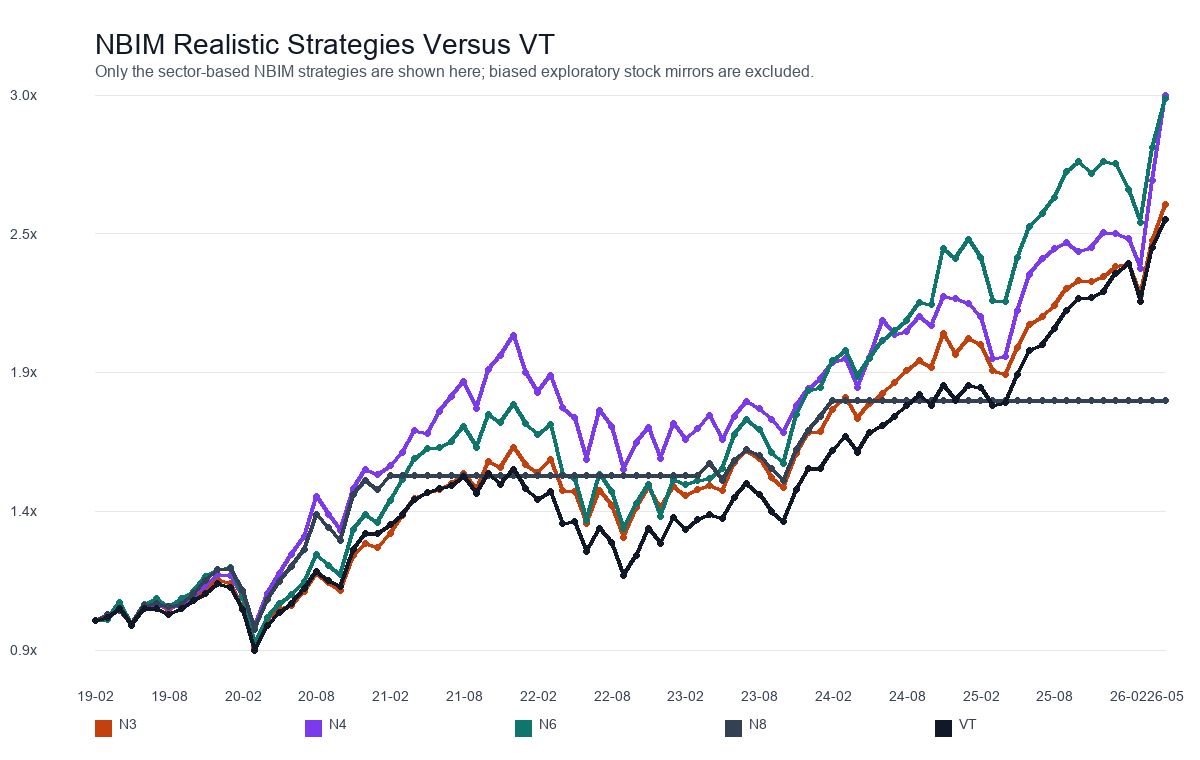
\includegraphics[width=0.92\textwidth]{nbim_realistic_nav_vs_vt.png}
\caption{NBIM sector-based strategies rebased against VT. Only the realistic industry strategies are shown; the exploratory direct mirror sleeve is intentionally excluded from this figure.}
\label{fig:nbim-nav}
\end{figure*}

\begin{figure}[!t]
\centering
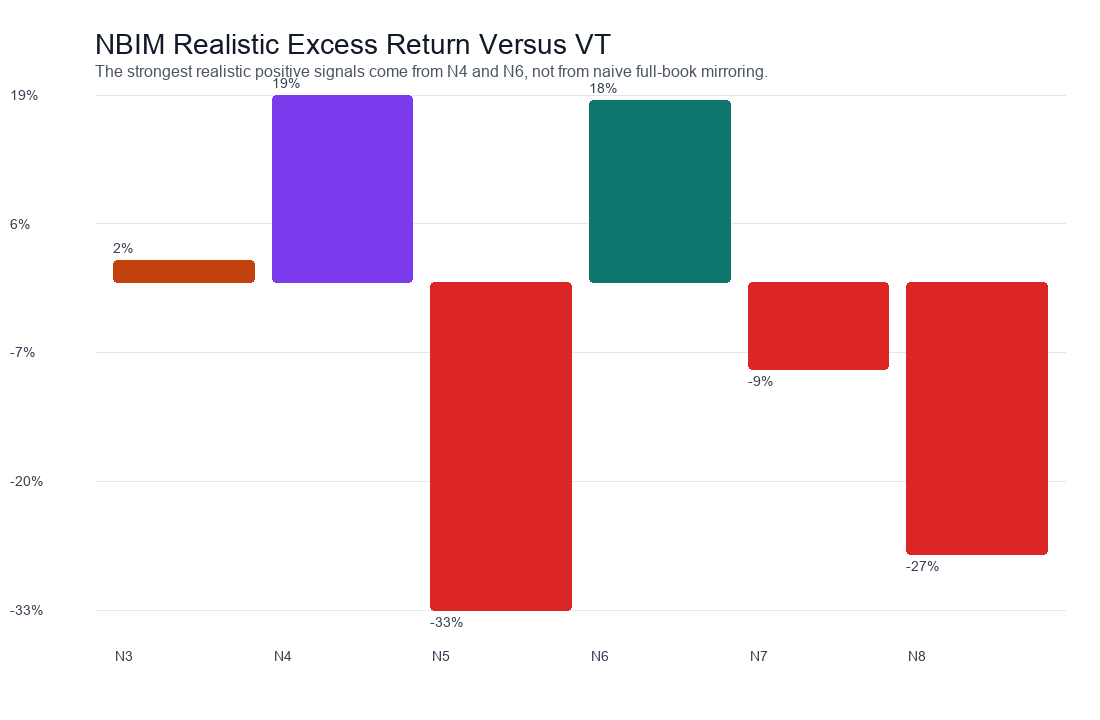
\includegraphics[width=\columnwidth]{nbim_realistic_excess_return.png}
\caption{Excess total return of realistic NBIM strategies versus VT.}
\label{fig:nbim-excess}
\end{figure}

\subsection{Why N1 and N2 Are Not Strong Alpha Evidence}

The most important NBIM result is not the high return of N1 and N2, but the reason that those returns cannot be treated as robust disclosure alpha. The mirror universe was a bounded U.S. mega-cap basket, and the bias audit showed that it overlapped almost perfectly with the top recurring U.S. names in the NBIM book across the sample. In other words, the backtest was effectively long a persistent basket of secular winners.

That is a valid exploratory result---it tells us what a bounded, disclosure-informed mega-cap sleeve would have done---but it is not clean evidence that the public disclosure stream itself creates a broadly harvestable copy-trading edge.

\subsection{What Looks More Credible}

The realistic NBIM findings are much narrower:
\begin{itemize}[leftmargin=1.4em]
    \item \textbf{N3} is essentially benchmark-like. Broadly mirroring NBIM's sector posture mostly reproduces a high-quality global allocation.
    \item \textbf{N4} is the strongest realistic signal. Following sectors whose disclosed weights increased produced a modest positive excess return of $18.6\%$ versus \texttt{VT}.
    \item \textbf{N6} also worked reasonably well. Concentrating on NBIM's top three sector exposures produced an $18.1\%$ excess return.
    \item \textbf{N5}, \textbf{N7}, and \textbf{N8} are weak or too sparse. Transition-only and consensus-only rules do not appear strong enough on their own in this implementation.
\end{itemize}

Thus, the most credible NBIM signal is not direct mirroring but slow-moving sector posture, especially disclosed industry weight change.

\section{Discussion}

\subsection{What the Combined Evidence Says}

The PIF and NBIM panels point to the same high-level conclusion from different directions:
\begin{itemize}[leftmargin=1.4em]
    \item direct single-name copy trading is weak once lag and partial visibility are respected;
    \item broad mirroring often collapses into benchmark-like exposure rather than differentiated alpha; and
    \item the most plausible residual signal lies in slower-moving allocation and sector rotation.
\end{itemize}

In PIF, even the most sensible copycat variant fails to beat \texttt{SPY}. In NBIM, the strongest realistic sector-based strategies are positive, but only modestly so.

\subsection{What Was Built Beyond the Final Returns}

This project produced more than terminal backtest numbers:
\begin{itemize}[leftmargin=1.4em]
    \item normalized holdings and transition datasets for PIF and NBIM;
    \item audit layers for disclosure dates, price coverage, and mirror-universe bias;
    \item benchmark-relative reports and chart packs;
    \item a PIF interactive explorer for stepping through filings, signals, orders, and portfolio evolution; and
    \item a reusable structure for extending the project to future monitoring and higher-capacity pricing sources.
\end{itemize}

This matters because disclosure-based alpha is especially vulnerable to hidden assumptions. The system-level outputs were designed to make those assumptions inspectable.

\section{Limitations}

Several limitations remain:
\begin{itemize}[leftmargin=1.4em]
    \item transaction costs and market impact were not modeled in the first-pass backtests;
    \item GIC was not included quantitatively because the public data was too incomplete;
    \item NBIM sector tests used U.S. ETF proxies for a global industry book, introducing representation error;
    \item the free-data path originally constrained NBIM timing, so the final implementation switched to a smaller Twelve Data daily proxy universe to obtain exact first-post-release execution;
    \item the strongest NBIM direct mirror results were contaminated by mirror-universe selection bias.
\end{itemize}

These do not invalidate the project, but they sharply limit how strong any alpha claim can be.

\section{Conclusion}

This study asked whether sovereign wealth fund disclosures can be monetized after realistic lag and visibility constraints are enforced. The answer is mostly negative for naive copy trading and only cautiously positive for narrow sector-based signals.

For PIF, no strategy generated alpha versus \texttt{SPY}. The best-performing design, cash-aware copying, improved materially on fully invested mirroring but still lagged passive beta.

For NBIM, the strongest raw stock-mirror result could not be accepted at face value because it was driven by a bounded basket of recurring mega-cap winners. More realistic industry-based strategies were far more credible, but the edge was modest. The best signals came from industry weight changes and concentrated leadership sectors, not from broad portfolio mirroring.

The highest-confidence conclusion is therefore:
\begin{quote}
\textit{Public SWF disclosures are more useful as slow-moving allocation and rotation signals than as literal copy-trading instructions.}
\end{quote}

The practical continuation of this research should prioritize monitoring tools, sector-rotation visualization, and higher-capacity price infrastructure, rather than ever-larger naive mirroring engines.

\section*{Artifact Note}

The paper corresponds to the committed project state pushed to the public repository at commit \texttt{2d51bd2}. The LaTeX source and figure assets in the local \texttt{paper/} directory were prepared after that push.

\begin{thebibliography}{99}

\bibitem{sec13f}
U.S. Securities and Exchange Commission, ``Frequently Asked Questions About Form 13F,'' \url{https://www.sec.gov/rules-regulations/staff-guidance/division-investment-management-frequently-asked-questions/frequently-asked-questions-about-form-13f}.

\bibitem{nbim}
Norges Bank Investment Management, ``Investments / All Investments,'' \url{https://www.nbim.no/en/investments/all-investments/}.

\bibitem{nbimholdings}
Norges Bank Investment Management, ``Terms of Use -- Holdings Data in Snowflake Marketplace,'' \url{https://www.nbim.no/en/terms-of-use-holdings-data-in-snowflake-marketplace/}.

\bibitem{gicreports}
GIC, ``Reports,'' \url{https://www.gic.com.sg/newsroom/reports/}.

\bibitem{gicsantiago}
GIC, ``Santiago Principles / Institutional Framework and Governance Structure,'' \url{https://www.gic.com.sg/how-we-invest/santiago-principles/institutional-framework-and-governance-structure/}.

\bibitem{alphavantage}
Alpha Vantage, ``Official Documentation,'' \url{https://www.alphavantage.co/documentation/}.

\bibitem{twelvedata}
Twelve Data, ``API Documentation,'' \url{https://twelvedata.com/docs}.

\end{thebibliography}

\end{document}
